\section{Triển khai Frontend}

Lớp giao diện người dùng (Frontend) của \textit{Secret Letter} được thiết kế dưới dạng ứng dụng trang đơn (Single Page Application - SPA), hướng tới mục tiêu tối ưu hóa trải nghiệm tương tác và hỗ trợ thực thi các tác vụ mật mã học trực tiếp trên trình duyệt web.

\subsection{Lựa chọn công nghệ cốt lõi}

Quá trình xây dựng Frontend được hiện thực hóa thông qua bộ công cụ phát triển hiện đại:
\begin{itemize}
    \item \textbf{React \& TypeScript:} Đảm nhận vai trò thiết lập kiến trúc giao diện phản ứng (Reactive UI). Việc sử dụng TypeScript kết hợp với cấu hình kiểm tra kiểu dữ liệu tĩnh giúp hạn chế đáng kể các rủi ro phát sinh lỗi thời gian thực (Runtime errors), đồng thời duy trì sự đồng bộ với các cấu trúc dữ liệu (Data models) đã được quy ước với Backend.
    \item \textbf{Vite:} Đóng vai trò là công cụ đóng gói (Build tool) thế hệ mới. Vite cung cấp cơ chế thay thế mô-đun nóng (Hot Module Replacement) giúp tăng tốc độ phát triển, đồng thời tối ưu hóa khối lượng mã nguồn tĩnh (Static assets) thông qua Rollup khi triển khai lên môi trường thực tế (Production).
\end{itemize}

\subsection{Triển khai mã hóa cục bộ (Client-Side Encryption)}

Đặc tính quan trọng nhất của dự án nằm ở việc hệ thống mã hóa được dịch chuyển hoàn toàn về phía thiết bị đầu cuối. Toàn bộ logic mật mã học được cô lập tại phân vùng \texttt{src/lib/crypto.ts}.

Thay vì phụ thuộc vào các thư viện mã hóa của bên thứ ba (như CryptoJS hay Forge), dự án khai thác trực tiếp bộ hàm \textbf{Web Crypto API} được tích hợp sẵn (Native) trên các trình duyệt hiện đại. Quyết định kỹ thuật này mang lại hai lợi thế lớn:
\begin{enumerate}
    \item \textbf{Tối ưu hiệu năng phần cứng:} Cho phép tiến trình mã hóa AES-GCM (256-bit) tận dụng trực tiếp sức mạnh xử lý thông qua các lệnh mã hóa cấp thấp của hệ điều hành, giúp các thao tác giải mã diễn ra mượt mà ngay cả trên thiết bị di động có cấu hình hạn chế.
    \item \textbf{Thu hẹp bề mặt tấn công:} Việc loại bỏ các thư viện mật mã của bên thứ ba giúp dự án thu hẹp đáng kể bề mặt tấn công chuỗi cung ứng (Supply Chain Attack) đối với luồng xử lý mã hóa cốt lõi.
\end{enumerate}

Trong quá trình vận hành, hàm \texttt{encryptSecret} chịu trách nhiệm tự động sinh ra một Nonce ngẫu nhiên dài 12-byte (bằng \texttt{crypto.getRandomValues}), sau đó kết hợp với khóa bí mật để biến đổi văn bản thuần (Plaintext) thành bản mã (Ciphertext) an toàn trước khi gửi đến máy chủ.

\subsection{Quản lý vòng đời luồng tương tác}

Kiến trúc hiển thị được phân chia rành mạch thành hai luồng màn hình chính, bám sát hai giai đoạn của một thông điệp:
\begin{itemize}
    \item \textbf{HomePage (Màn hình Khởi tạo):} Đảm nhận việc tiếp nhận dữ liệu đầu vào. Trạng thái biểu mẫu (Form State) được thiết lập để kiểm soát chặt chẽ dung lượng văn bản (giới hạn tối đa 10KB). 
    
    \begin{figure}[H]
        \centering
        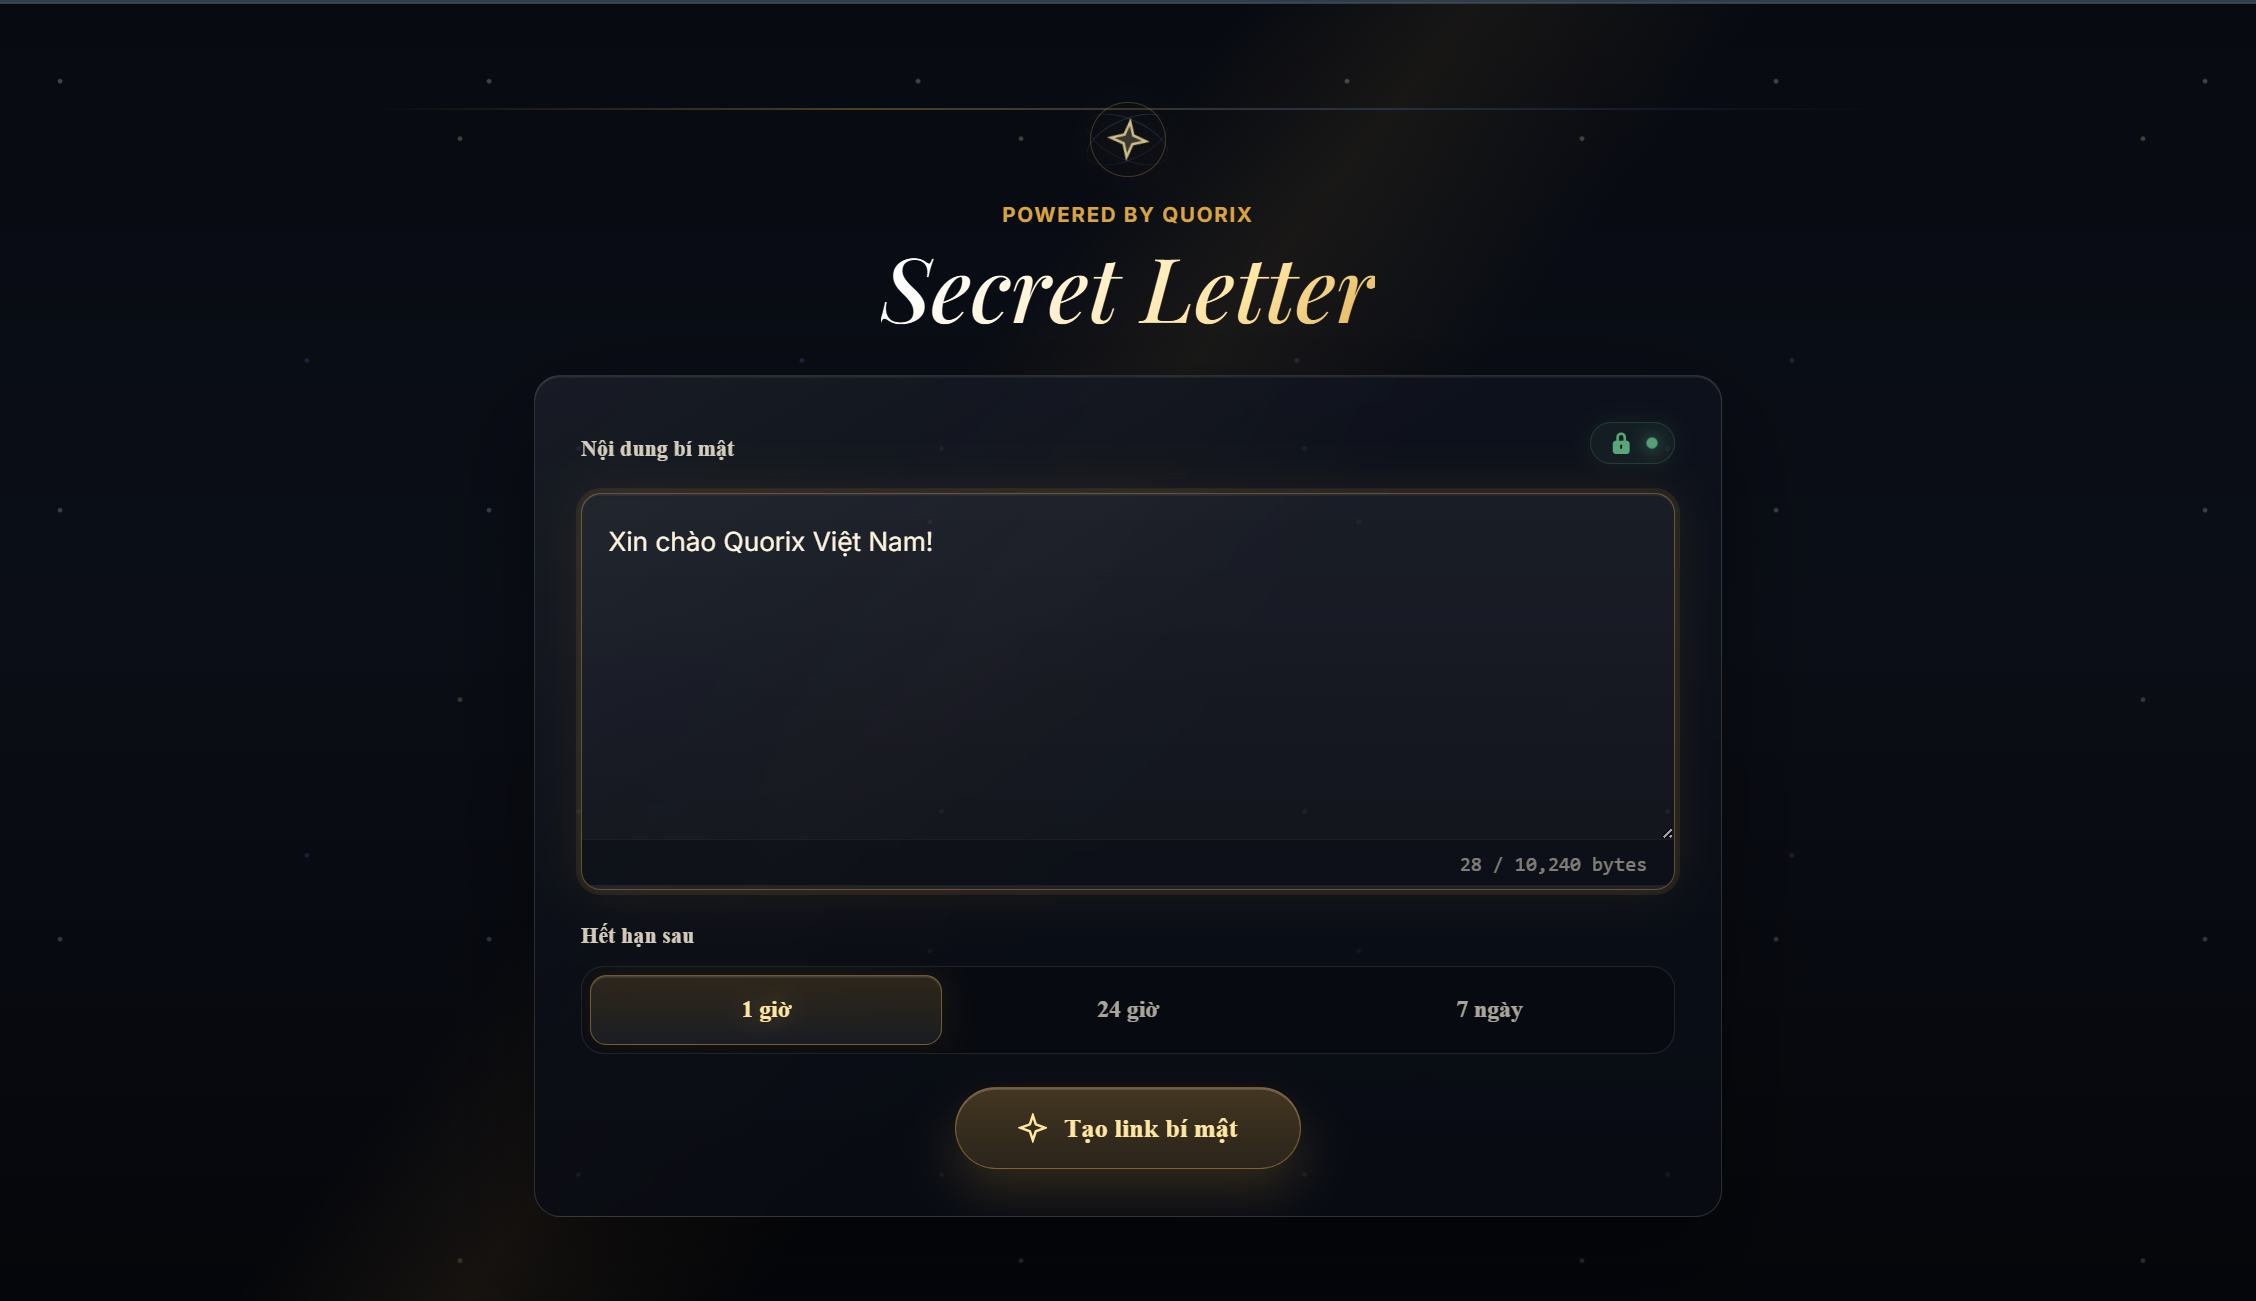
\includegraphics[width=0.8\textwidth]{img/ui_home_create.png}
        \caption[Giao diện soạn thảo thông điệp và cấu hình TTL]{Giao diện soạn thảo thông điệp và cấu hình thời gian sống (TTL)}
        \label{fig:ui_home_create}
    \end{figure}
    
    Khi người dùng tiến hành mã hóa, Frontend sẽ gọi API \texttt{POST /api/secrets} và chỉ cấp phát liên kết an toàn (Secret Link) khi máy chủ đã xác nhận lưu trữ bản mã thành công.

    \begin{figure}[H]
        \centering
        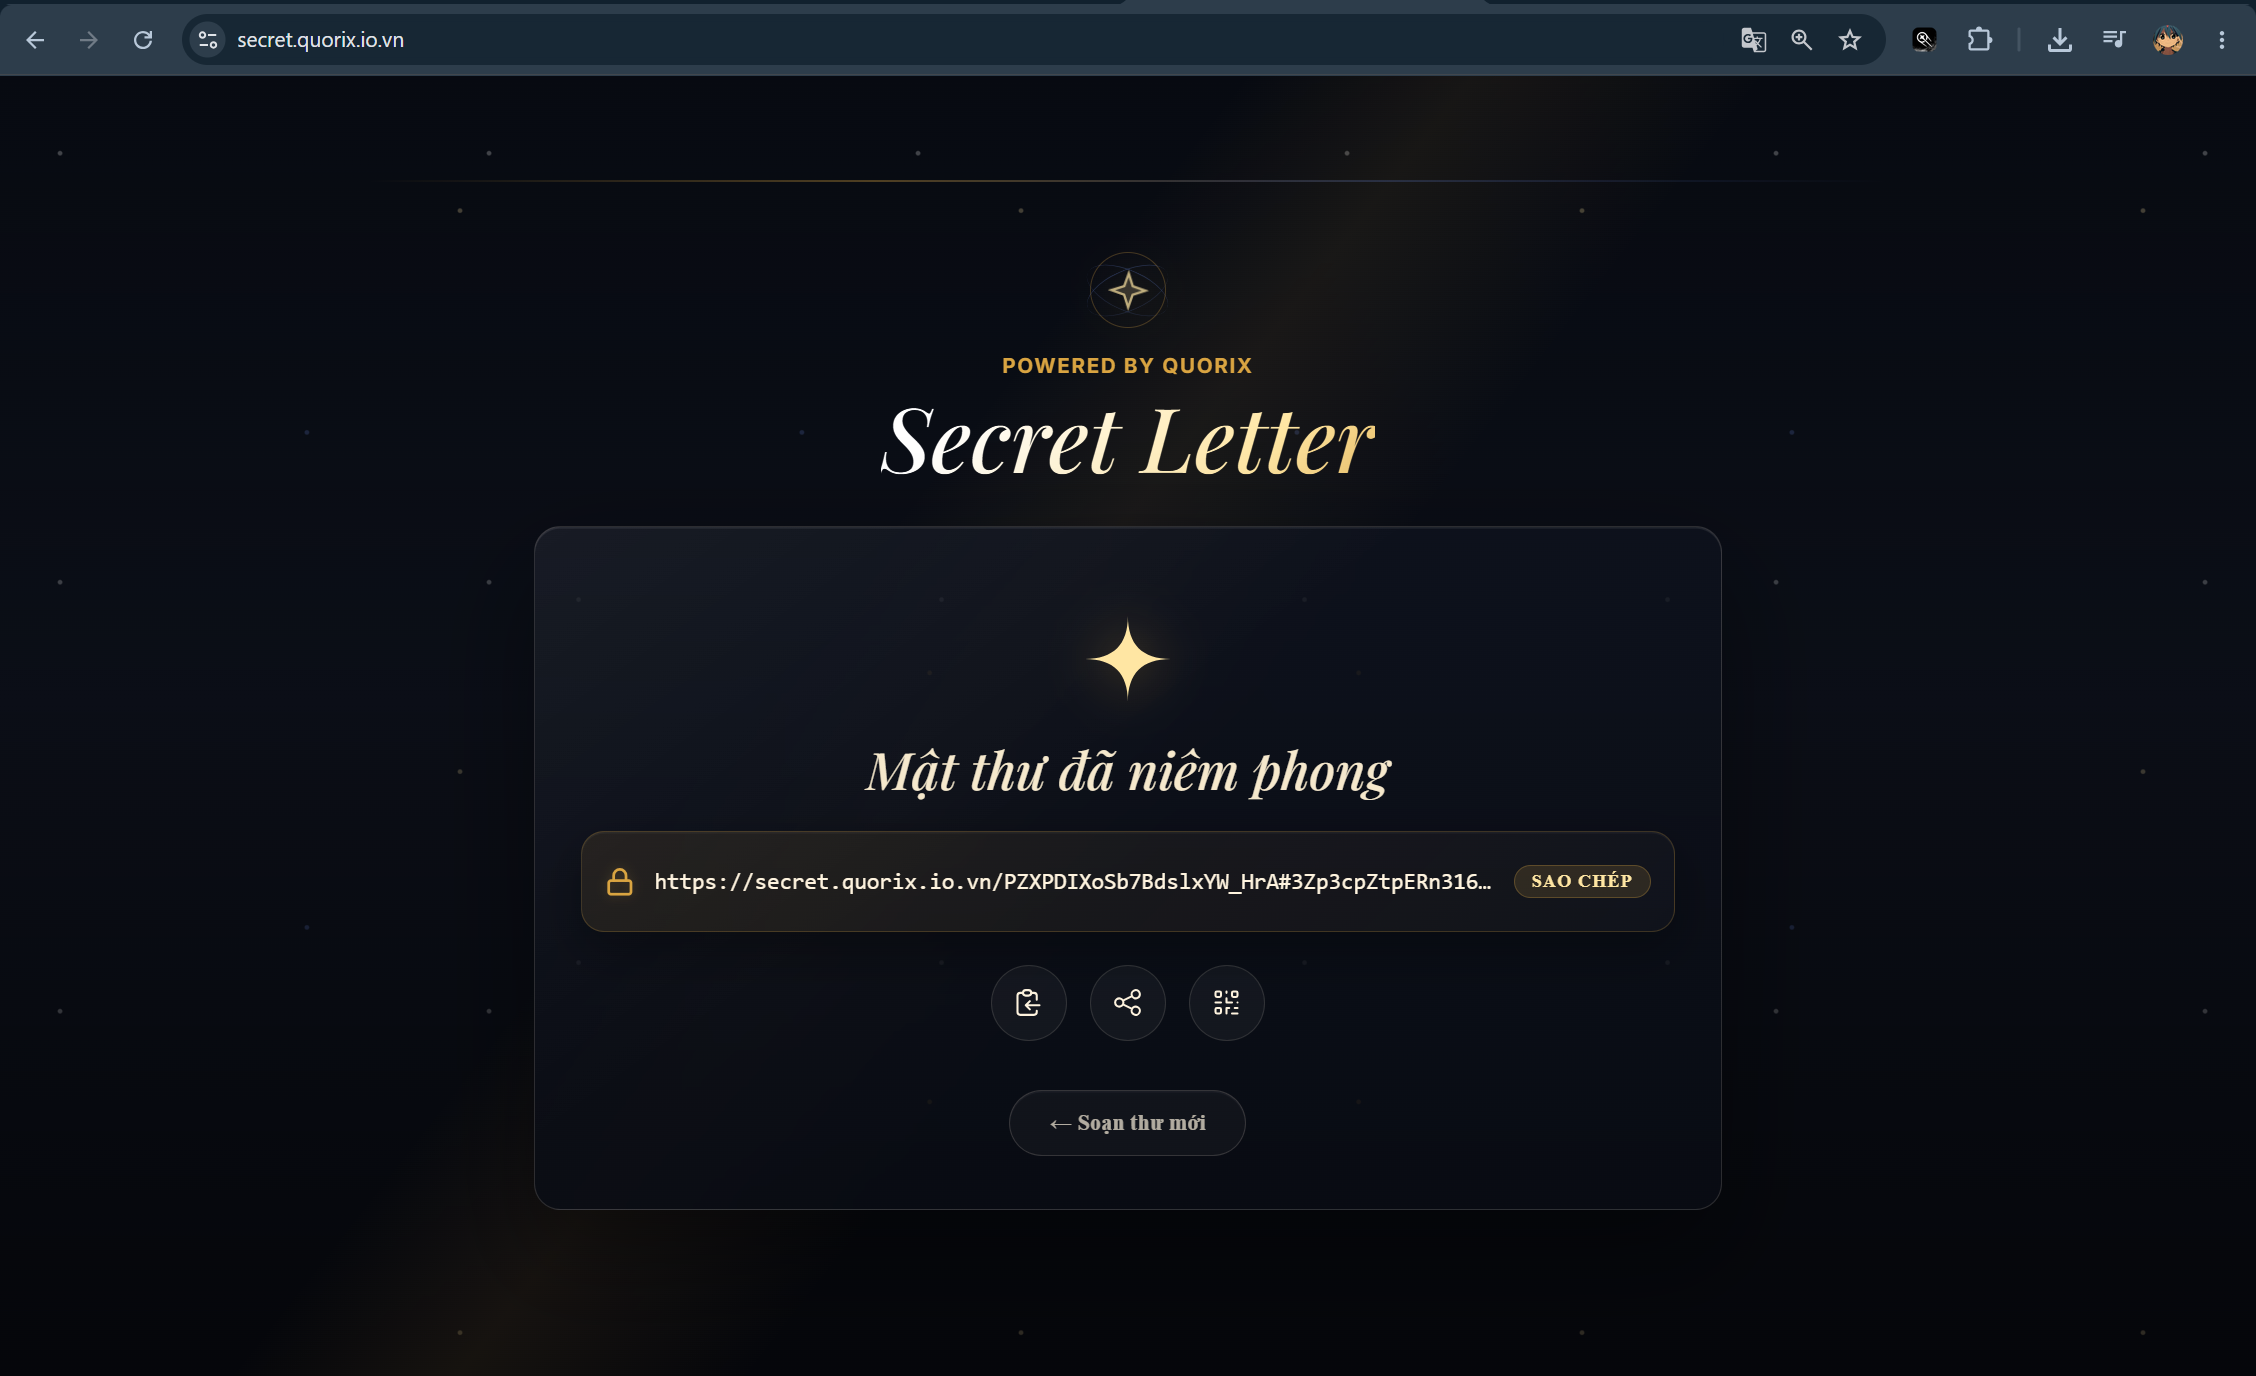
\includegraphics[width=0.8\textwidth]{img/ui_home_link.png}
        \caption[Trạng thái liên kết an toàn sau mã hóa]{Trạng thái trả về liên kết an toàn sau khi mã hóa thành công}
        \label{fig:ui_home_link}
    \end{figure}

    \item \textbf{RevealPage (Màn hình Giải mã):} Đảm nhận luồng kiểm duyệt và chống tự động hóa (Anti-Bot). Khi người nhận truy cập thông qua liên kết (chứa khóa giải mã tại đoạn \texttt{\#key=...}), hệ thống không tự ý tải bản mã về. Thay vào đó, giao diện sẽ thiết lập một phiên giao dịch ngắn hạn (Reveal Session) và yêu cầu người dùng thao tác vật lý (nhấn nút "Mở thư"). 

    \begin{figure}[H]
        \centering
        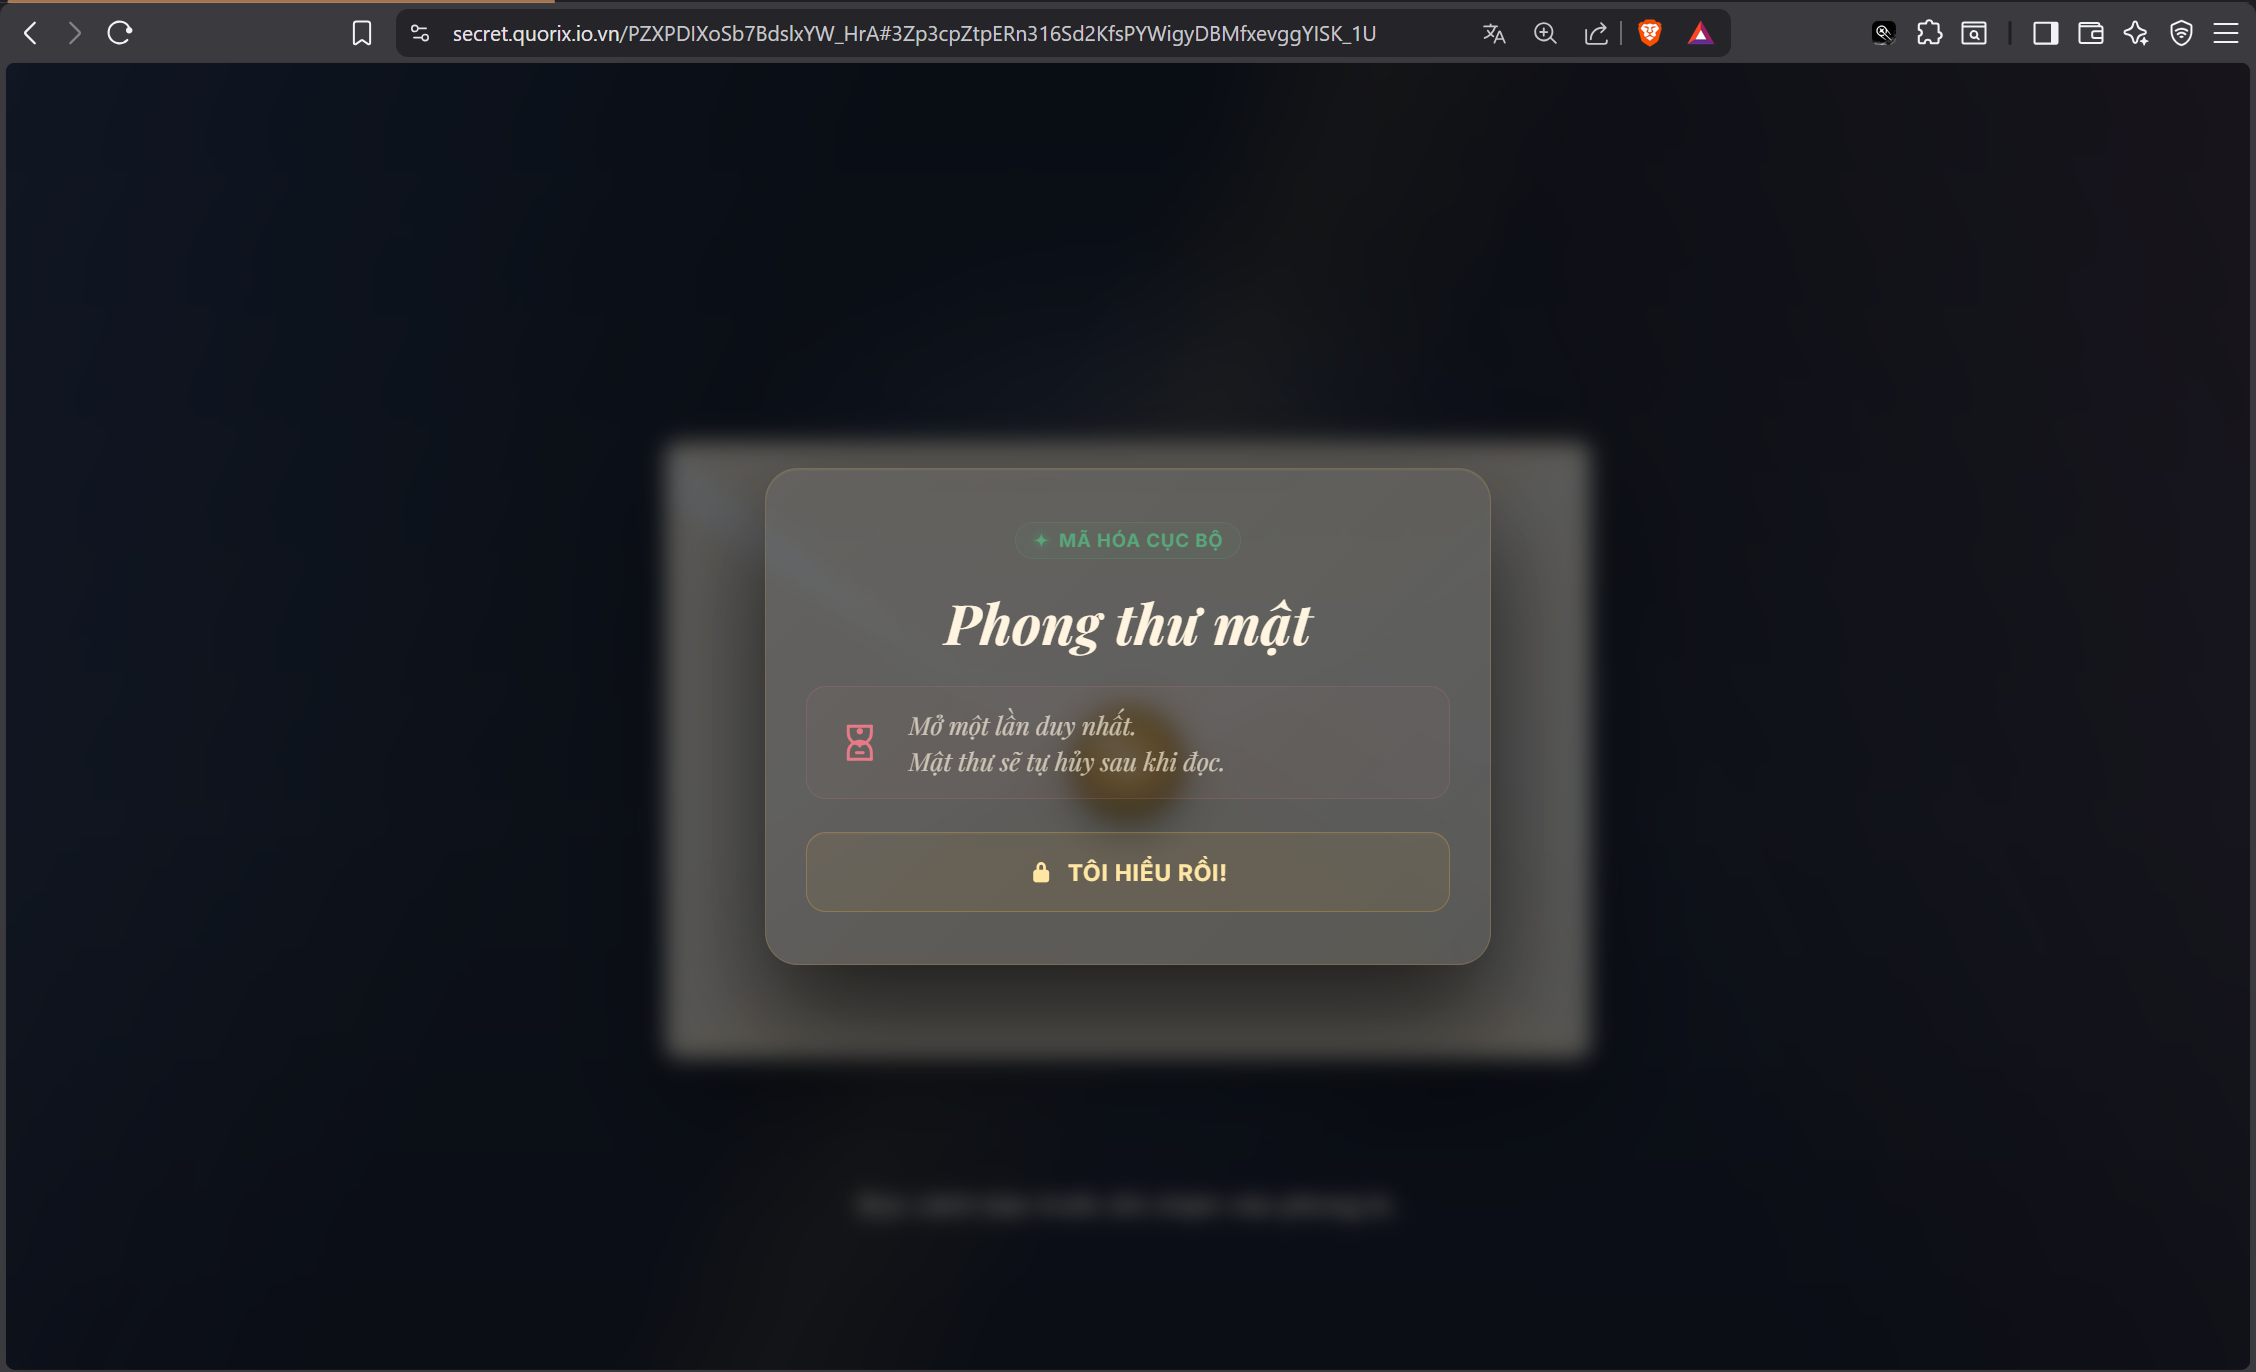
\includegraphics[width=0.8\textwidth]{img/ui_reveal_gate.png}
        \caption[Giao diện Anti-Bot xác thực tương tác vật lý]{Giao diện Anti-Bot buộc người nhận phải tương tác vật lý}
        \label{fig:ui_reveal_gate}
    \end{figure}

    Chỉ sau khi vượt qua rào cản này, văn bản mã hóa mới được trích xuất từ Redis, trả về trình duyệt và phục hồi thông qua hàm \texttt{decryptSecret}.

    \begin{figure}[H]
        \centering
        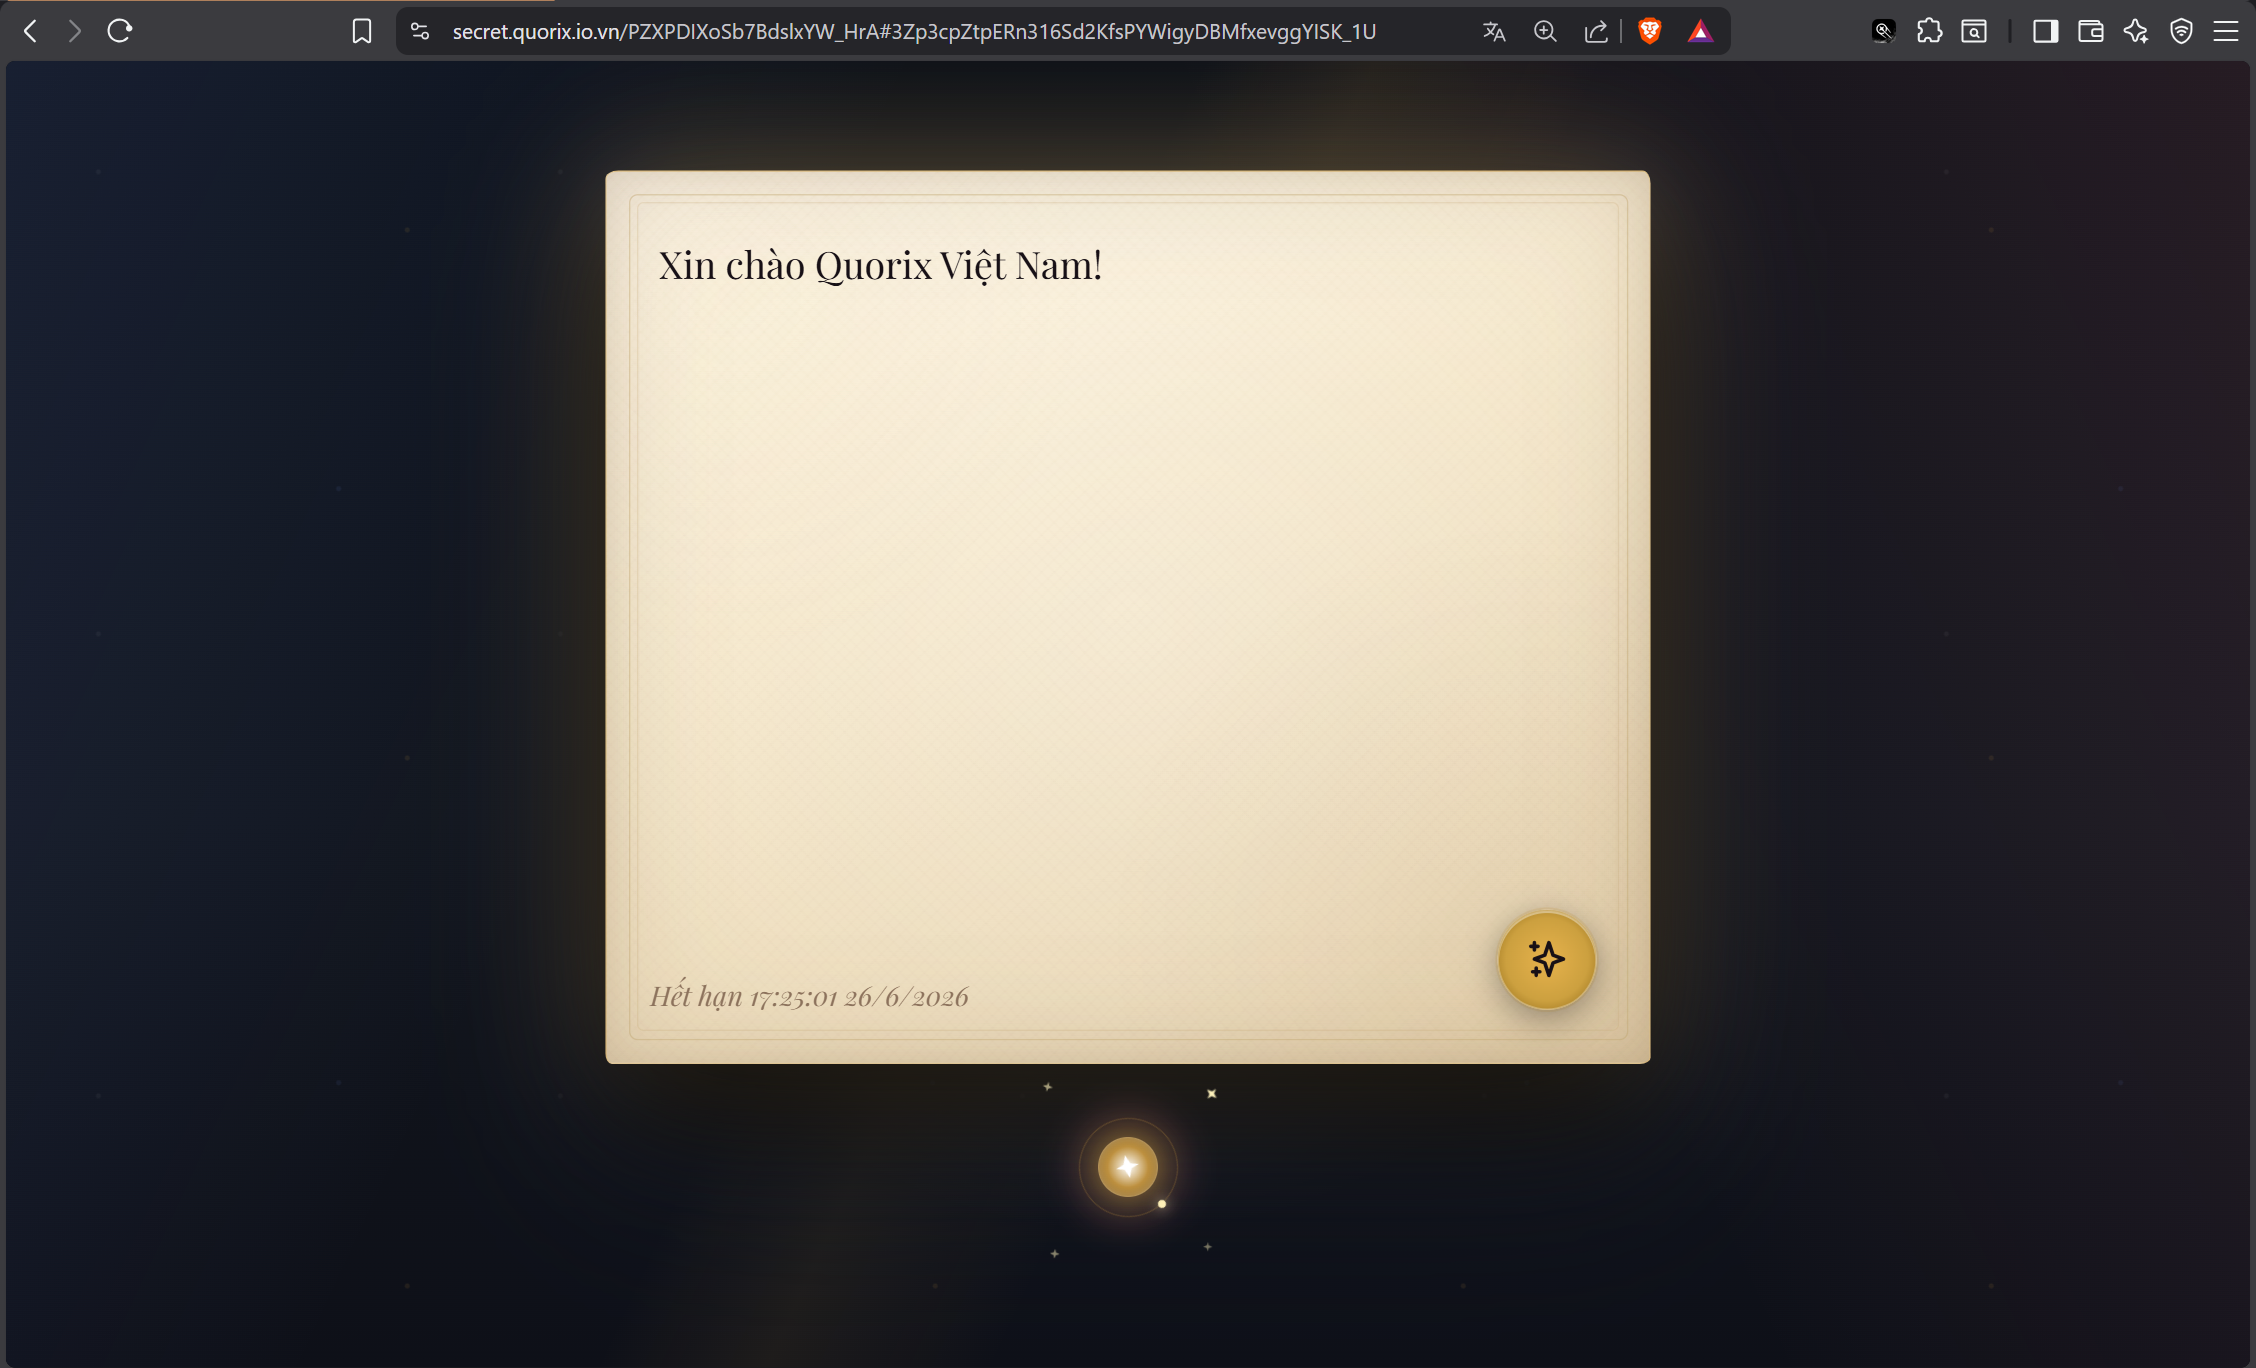
\includegraphics[width=0.8\textwidth]{img/ui_reveal_decrypted.png}
        \caption[Giao diện hiển thị nội dung thông điệp sau giải mã]{Giao diện hiển thị nội dung thông điệp sau khi giải mã thành công}
        \label{fig:ui_reveal_decrypted}
    \end{figure}

    Ngay sau khi thông điệp được giải mã và hiển thị, bản ghi trên máy chủ Redis sẽ lập tức bị xóa bỏ. Nếu người dùng vô tình tải lại trang hoặc truy cập lại liên kết, hệ thống sẽ thông báo lá thư đã bị tiêu hủy, hoàn tất vòng đời "Burn-after-reading" (Hình \ref{fig:ui_reveal_destroyed}).

    \begin{figure}[H]
        \centering
        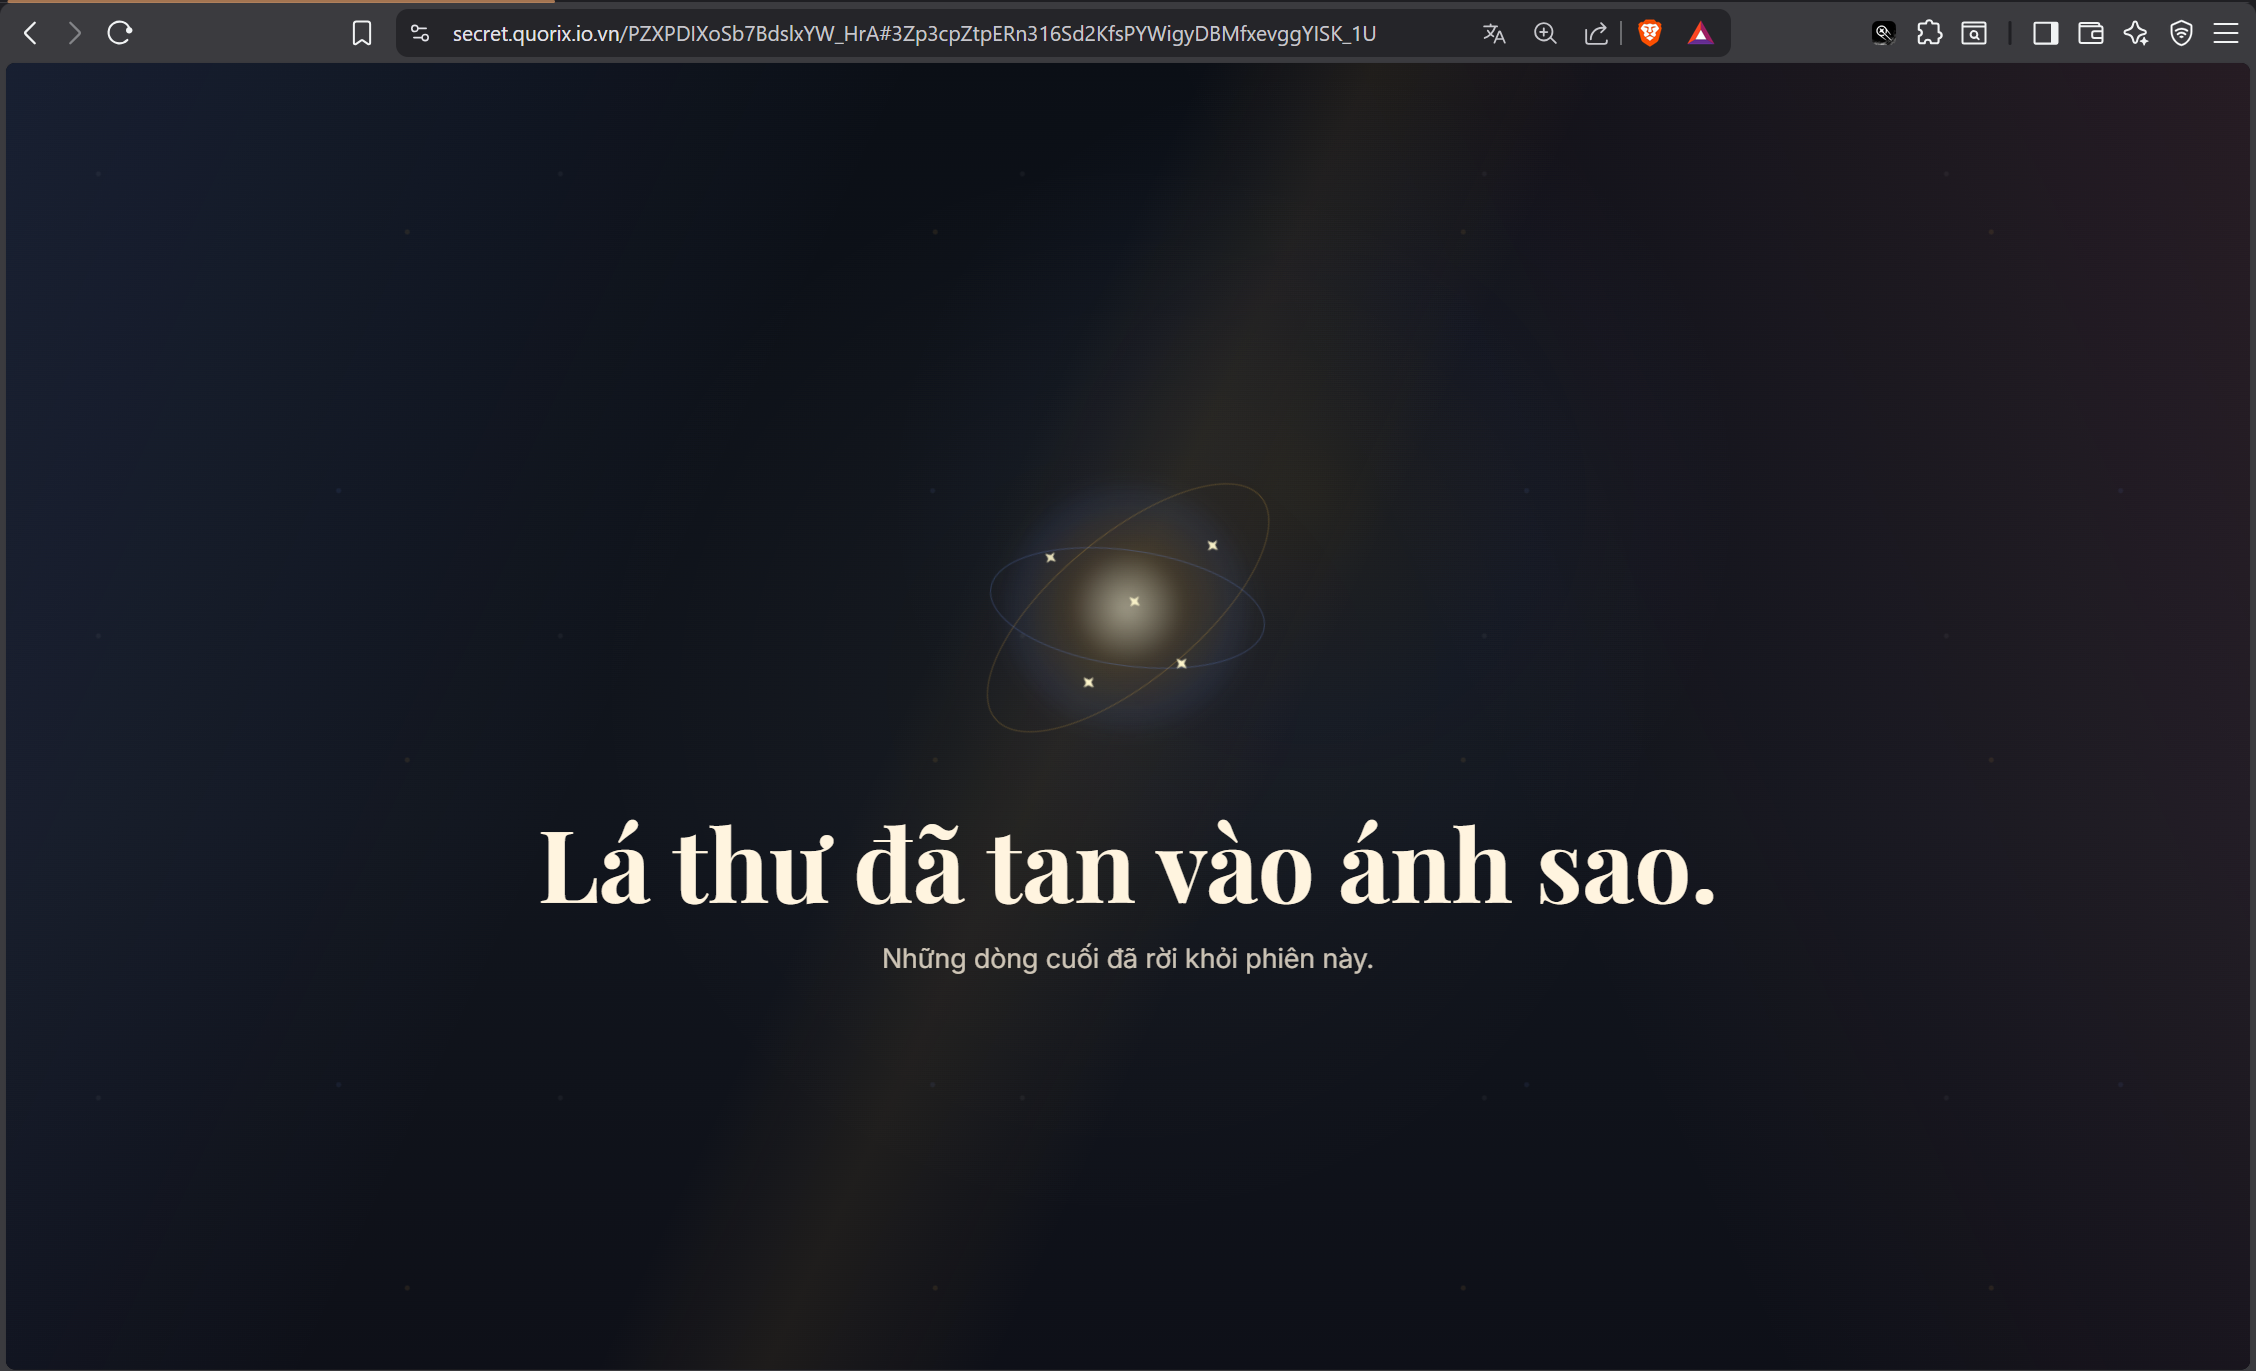
\includegraphics[width=0.8\textwidth]{img/ui_reveal_destroyed.png}
        \caption[Giao diện thông báo thư bị hủy vĩnh viễn]{Giao diện thông báo lá thư đã bị huỷ vĩnh viễn}
        \label{fig:ui_reveal_destroyed}
    \end{figure}

    \item \textbf{Xử lý ngoại lệ (Error Boundaries):} Nhằm đảm bảo trải nghiệm người dùng, Frontend cung cấp các phản hồi thị giác rõ ràng khi luồng giải mã gặp sự cố. Điển hình là việc nhận diện các truy cập thiếu tham số khóa mã hóa (Missing Key), hoặc khóa không hợp lệ (Wrong Key) dẫn đến thất bại trong việc giải mã.

    \begin{figure}[H]
        \centering
        \begin{minipage}{0.48\textwidth}
            \centering
            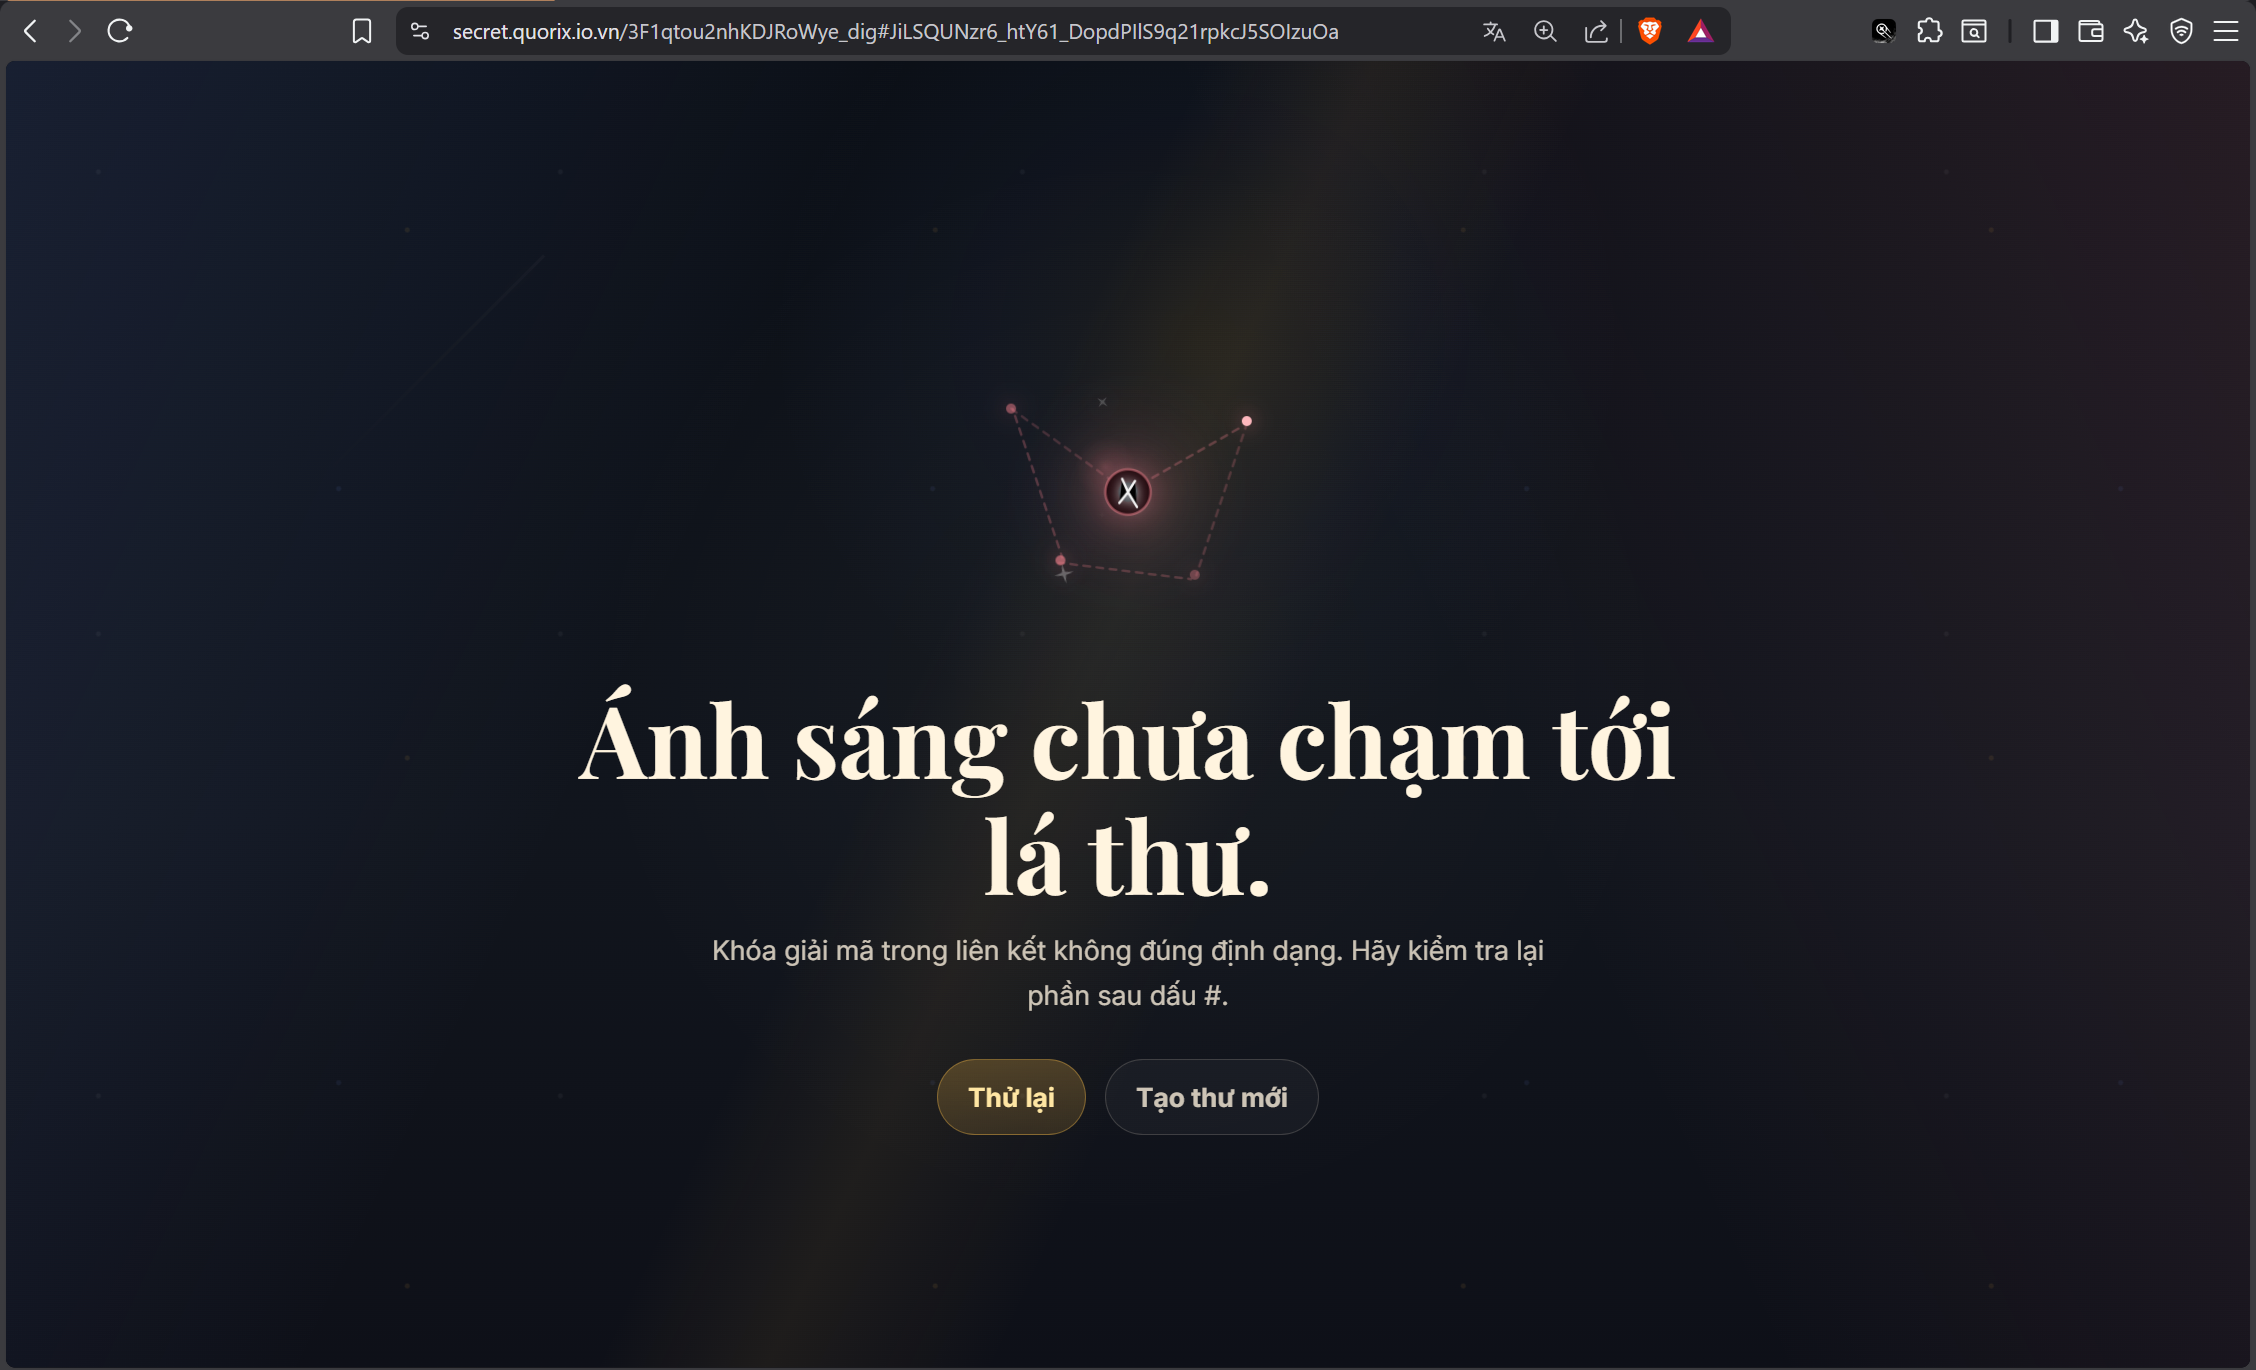
\includegraphics[width=\linewidth]{img/ui_error_nokey.png}
            \caption[Cảnh báo khi liên kết thiếu đoạn khóa]{Cảnh báo khi liên kết thiếu đoạn khóa}
            \label{fig:ui_error_nokey}
        \end{minipage}\hfill
        \begin{minipage}{0.48\textwidth}
            \centering
            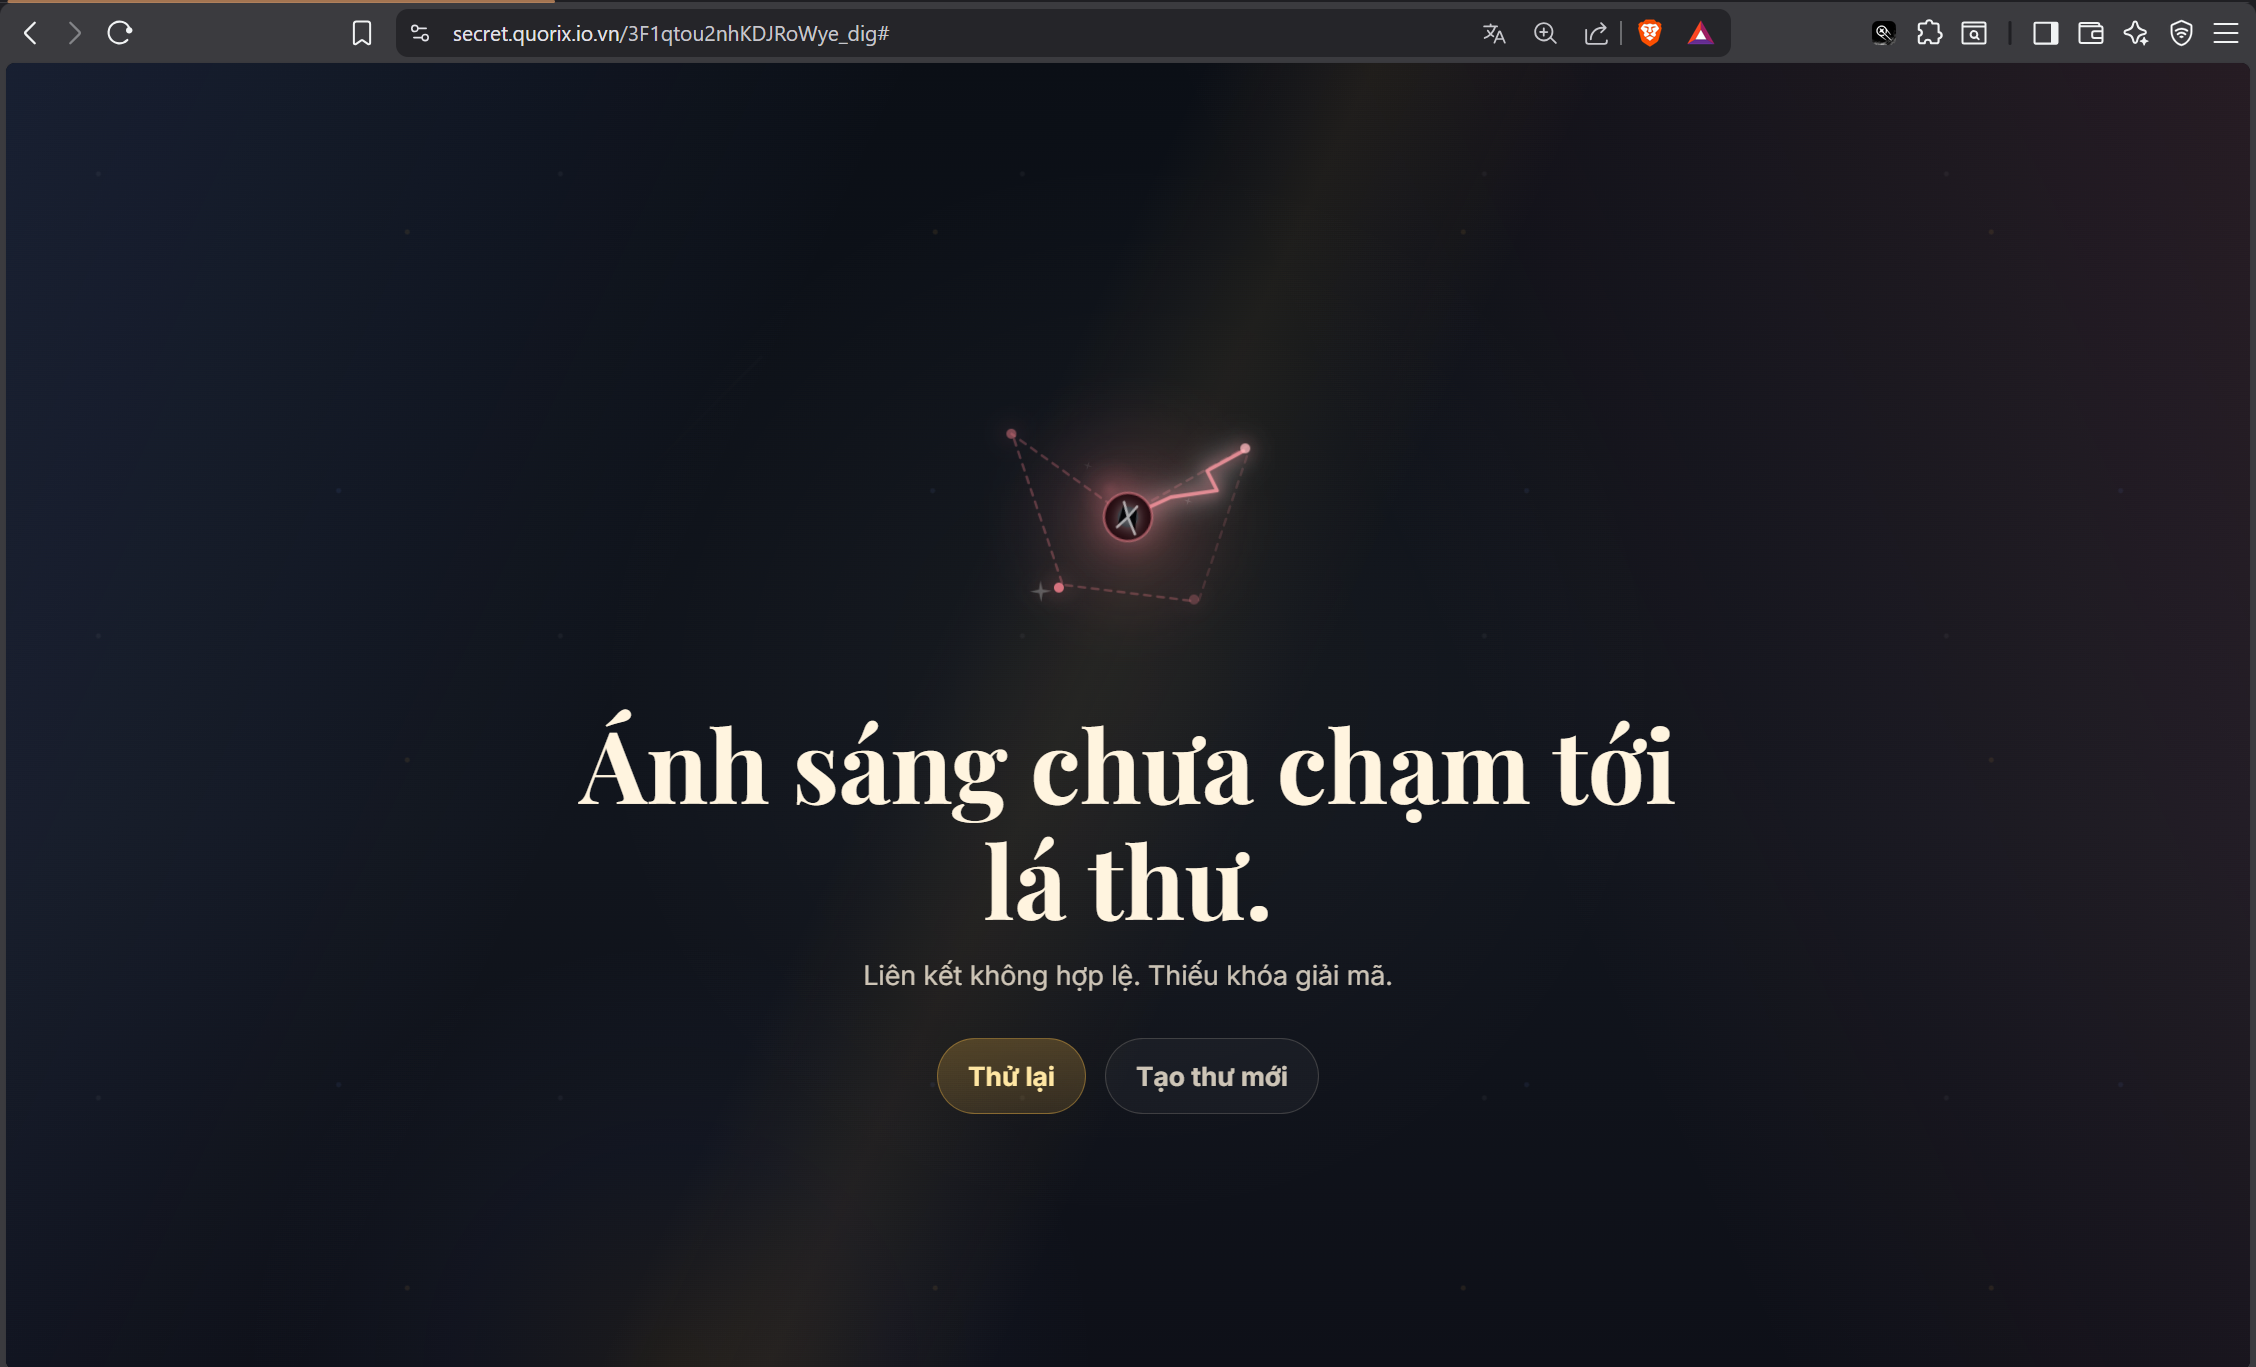
\includegraphics[width=\linewidth]{img/ui_error_wrongkey.png}
            \caption[Cảnh báo khi giải mã thất bại do sai khóa]{Cảnh báo khi giải mã thất bại do sai khóa}
            \label{fig:ui_error_wrongkey}
        \end{minipage}
    \end{figure}
\end{itemize}